%  LaTeX support: latex@mdpi.com
%  For support, please attach all files needed for compiling as well as the log file, and specify your operating system, LaTeX version, and LaTeX editor.

%=================================================================
\documentclass[energies,article,submit,pdftex,moreauthors]{Definitions/mdpi}
%\documentclass[preprints,article,submit,pdftex,moreauthors]{Definitions/mdpi}
% For posting an early version of this manuscript as a preprint, you may use "preprints" as the journal. Changing "submit" to "accept" before posting will remove line numbers.

% Below journals will use APA reference format:
% admsci, aieduc, behavsci, businesses, econometrics, economies, education, ejihpe, famsci, games, humans, ijcs, ijfs, journalmedia, jrfm, languages, psycholint, publications, tourismhosp, youth

% Below journals will use Chicago reference format:
% arts, genealogy, histories, humanities, jintelligence, laws, literature, religions, risks, socsci

%--------------------
% Class Options:
%--------------------
%----------
% journal
%----------
% Choose between the following MDPI journals:
% energies

%---------
% article
%---------
% The default type of manuscript is "article"
% supfile = supplementary materials

%----------
% submit
%----------
% The class option "submit" will be changed to "accept" by the Editorial Office when the paper is accepted. This will only make changes to the frontpage (e.g., the logo of the journal will get visible), the headings, and the copyright information. Also, line numbering will be removed. Journal info and pagination for accepted papers will also be assigned by the Editorial Office.

%------------------
% moreauthors
%------------------
% If there is only one author the class option oneauthor should be used. Otherwise use the class option moreauthors.

%---------
% pdftex
%---------
% The option pdftex is for use with pdfLaTeX. Remove "pdftex" for (1) compiling with LaTeX & dvi2pdf (if eps figures are used) or for (2) compiling with XeLaTeX.

%=================================================================
% MDPI internal commands - do not modify
\firstpage{1}
\makeatletter
\setcounter{page}{\@firstpage}
\makeatother
\pubvolume{1}
\issuenum{1}
\articlenumber{0}
\pubyear{2025}
\copyrightyear{2025}
%\externaleditor{Firstname Lastname} % More than 1 editor, please add `` and '' before the last editor name
\datereceived{ }
\daterevised{ } % Comment out if no revised date
\dateaccepted{ }
\datepublished{ }
%\datecorrected{} % For corrected papers: "Corrected: XXX" date in the original paper.
%\dateretracted{} % For retracted papers: "Retracted: XXX" date in the original paper.
\hreflink{https://doi.org/} % If needed use \linebreak
%\doinum{}
%\pdfoutput=1 % Uncommented for upload to arXiv.org
%\CorrStatement{yes}  % For updates
%\longauthorlist{yes} % For many authors that exceed the left citation part

%=================================================================
% Add packages and commands here. The following packages are loaded in our class file: fontenc, inputenc, calc, indentfirst, fancyhdr, graphicx, epstopdf, lastpage, ifthen, float, amsmath, amssymb, lineno, setspace, enumitem, mathpazo, booktabs, titlesec, etoolbox, tabto, xcolor, colortbl, soul, multirow, microtype, tikz, totcount, changepage, attrib, upgreek, array, tabularx, pbox, ragged2e, tocloft, marginnote, marginfix, enotez, amsthm, natbib, hyperref, cleveref, scrextend, url, geometry, newfloat, caption, draftwatermark, seqsplit
% cleveref: load \crefname definitions after \begin{document}

%=================================================================
% Please use the following mathematics environments: Theorem, Lemma, Corollary, Proposition, Characterization, Property, Problem, Example, ExamplesandDefinitions, Hypothesis, Remark, Definition, Notation, Assumption
%% For proofs, please use the proof environment (the amsthm package is loaded by the MDPI class).

%=================================================================
% Full title of the paper (Capitalized)
\Title{Material exergy}

% MDPI internal command: Title for citation in the left column
\TitleCitation{Material exergy}

% Author Orchid ID: enter ID or remove command
\newcommand{\orcidauthorA}{0000-0000-0000-000X} % Add \orcidA{} behind the author's name
\newcommand{\orcidauthorB}{0000-0000-0000-000X} % Add \orcidB{} behind the author's name
\newcommand{\orcidauthorC}{0000-0002-7438-214X} % Add \orcidC{} behind the author's name
\newcommand{\orcidauthorD}{0000-0000-0000-000X} % Add \orcidD{} behind the author's name

% Authors, for the paper (add full first names)
\Author{Erin Schuman $^{1,\dagger}$\orcidA{},
        Sofie Schumerth $^{2,\dagger}$\orcidB{},
        Matthew Kuperus Heun $^{3,}$*\orcidC{}, and
        Tania Sousa $^{4}$\orcidD{} }

%\longauthorlist{yes}

% MDPI internal command: Authors, for metadata in PDF
\AuthorNames{Erin Schuman,
             Sofie Schumerth,
             Matthew Kuperus Heun, and
             Tania Sousa}

% MDPI internal command: Authors, for citation in the left column, only choose below one of them according to the journal style
% If this is a Chicago style journal
% (arts, genealogy, histories, humanities, jintelligence, laws, literature, religions, risks, socsci):
% Lastname, Firstname, Firstname Lastname, and Firstname Lastname.

% If this is a APA style journal
% (admsci, behavsci, businesses, econometrics, economies, education, ejihpe, games, humans, ijfs, journalmedia, jrfm, languages, psycholint, publications, tourismhosp, youth):
% Lastname, F., Lastname, F., \& Lastname, F.

% If this is a ACS style journal (Except for the above Chicago and APA journals, all others are in the ACS format):
% Lastname, F.; Lastname, F.; Lastname, F.
\isAPAStyle{%
       \AuthorCitation{Schuman, E., Schumerth, S., Heun, M.K., \& Sousa, T.}
         }{%
\isChicagoStyle{%
        \AuthorCitation{Schuman, Erin, Sofie Schumerth, Matthew Kuperus Heun, and Tania Sousa.}
        }{
        \AuthorCitation{Schuman, E.; Schumerth, S.; Heun, M.K.; Sousa, T.}
        }
}

% Affiliations / Addresses (Add [1] after \address if there is only one affiliation.)
% \address{%
% $^{1}$ \quad Affiliation 1; e-mail@e-mail.com\\
% $^{2}$ \quad Affiliation 2; e-mail@e-mail.com}
\address{%
$^{1}$ \quad Engineering Department, Calvin University, 3201 Burton St.\ SE, Grand Rapids, MI, USA, ees44@calvin.edu\\
$^{2}$ \quad Engineering Department, Calvin University, 3201 Burton St.\ SE, Grand Rapids, MI, USA, sis2@calvin.edu\\
$^{3}$ \quad Engineering Department, Calvin University, 3201 Burton St.\ SE, Grand Rapids, MI, USA, mkh2@calvin.edu;
             Sustainability Research Institute, School of Earth and Environment, University of Leeds, Leeds, UK;
             School for Public Leadership, Faculty of Economic and Management Science, Stellenbosch University, Stellenbosch, South Africa \\
$^{4}$ \quad MARETEC—Marine, Environment and Technology Center, LARSyS, Instituto Superior T\'{e}cnico, Universidade de Lisboa, Avenida Rovisco Pais, 1, Lisboa, Portugal, taniasousa@tecnico.ulisboa.pt}


% Contact information of the corresponding author
\corres{Corresponding author: mkh2@calvin.ed, +1 (616) 526-6663}

% Current address and/or shared authorship
% \firstnote{Current address: Affiliation.}  % Current address should not be the same as any items in the Affiliation section.
\firstnote{These authors contributed equally to this work.}
% The commands \secondnote{} till \eighthnote{} are available for further notes

%\simplesumm{} % Simple summary

%\conference{} % An extended version of a conference paper

% Abstract (Do not insert blank lines, i.e. \\)
\abstract{A single paragraph of about 200 words maximum. For research articles, abstracts should give a pertinent overview of the work. We strongly encourage authors to use the following style of structured abstracts, but without headings: (1) Background: place the question addressed in a broad context and highlight the purpose of the study; (2) Methods: describe briefly the main methods or treatments applied; (3) Results: summarize the article's main findings; (4) Conclusions: indicate the main conclusions or interpretations. The abstract should be an objective representation of the article, it must not contain results which are not presented and substantiated in the main text and should not exaggerate the main conclusions.}

% Keywords
\keyword{keyword 1; keyword 2; keyword 3 (List three to ten pertinent keywords specific to the article; yet reasonably common within the subject discipline.)}

% The fields PACS, MSC, and JEL may be left empty or commented out if not applicable
%\PACS{J0101}
%\MSC{}
%\JEL{}

%%%%%%%%%%%%%%%%%%%%%%%%%%%%%%%%%%%%%%%%%%
% Only for the journal Diversity
%\LSID{\url{http://}}

%%%%%%%%%%%%%%%%%%%%%%%%%%%%%%%%%%%%%%%%%%
% Only for the journal Applied Sciences
%\featuredapplication{Authors are encouraged to provide a concise description of the specific application or a potential application of the work. This section is not mandatory.}
%%%%%%%%%%%%%%%%%%%%%%%%%%%%%%%%%%%%%%%%%%

%%%%%%%%%%%%%%%%%%%%%%%%%%%%%%%%%%%%%%%%%%
% Only for the journal Data
%\dataset{DOI number or link to the deposited data set if the data set is published separately. If the data set shall be published as a supplement to this paper, this field will be filled by the journal editors. In this case, please submit the data set as a supplement.}
%\datasetlicense{License under which the data set is made available (CC0, CC-BY, CC-BY-SA, CC-BY-NC, etc.)}

%%%%%%%%%%%%%%%%%%%%%%%%%%%%%%%%%%%%%%%%%%
% Only for the journal BioTech, Fishes, Neuroimaging and Toxins
%\keycontribution{The breakthroughs or highlights of the manuscript. Authors can write one or two sentences to describe the most important part of the paper.}

%%%%%%%%%%%%%%%%%%%%%%%%%%%%%%%%%%%%%%%%%%
% Only for the journal Encyclopedia
%\encyclopediadef{For entry manuscripts only: please provide a brief overview of the entry title instead of an abstract.}

%%%%%%%%%%%%%%%%%%%%%%%%%%%%%%%%%%%%%%%%%%
% Only for the journal Advances in Respiratory Medicine, Future, Sensors and Smart Cities
%\addhighlights{yes}
%\renewcommand{\addhighlights}{%
%
%\noindent This is an obligatory section in ``Advances in Respiratory Medicine'', ``Future'', ``Sensors'' and ``Smart Cities”, whose goal is to increase the discoverability and readability of the article via search engines and other scholars. Highlights should not be a copy of the abstract, but a simple text allowing the reader to quickly and simplified find out what the article is about and what can be cited from it. Each of these parts should be devoted up to 2~bullet points.\vspace{3pt}\\
%\textbf{What are the main findings?}
% \begin{itemize}[labelsep=2.5mm,topsep=-3pt]
% \item First bullet.
% \item Second bullet.
% \end{itemize}\vspace{3pt}
%\textbf{What is the implication of the main finding?}
% \begin{itemize}[labelsep=2.5mm,topsep=-3pt]
% \item First bullet.
% \item Second bullet.
% \end{itemize}
%}

%%%%%%%%%%%%%%%%%%%%%%%%%%%%%%%%%%%%%%%%%%
\begin{document}

%%%%%%%%%%%%%%%%%%%%%%%%%%%%%%%%%%%%%%%%%%


%%%%%%%%%%%%%%%%%%%%%%%%%%%%%%%%%%%%%%%%%%%%%%%%%%%%%%%%%%%%%%
\section{Introduction}
\label{sec:introduction}
%%%%%%%%%%%%%%%%%%%%%%%%%%%%%%%%%%%%%%%%%%%%%%%%%%%%%%%%%%%%%%

% The introduction should briefly place the study in a broad context and highlight why it is important. It should define the purpose of the work and its significance. The current state of the research field should be reviewed carefully and key publications cited. Please highlight controversial and diverging hypotheses when necessary. Finally, briefly mention the main aim of the work and highlight the principal conclusions. As far as possible, please keep the introduction comprehensible to scientists outside your particular field of research. Citing a journal paper \citep{ref-journal}.  Now citing a book reference \citep{ref-book1,ref-book2} or other reference types \citep{ref-unpublish,ref-url}. Please use the command \citep{ref-proceeding,ref-thesis} for the following MDPI journals, which use author--date citation: Administrative Sciences, Arts, Behavioral Sciences, Businesses, Econometrics, Economies, Education Sciences, European Journal of Investigation in Health, Psychology and Education, Games, Genealogy, Histories, Humanities, Humans, IJFS, Journal of Intelligence, Journalism and Media, JRFM, Languages, Laws, Literature, Psychology International, Publications, Religions, Risks, Social Sciences, Tourism and Hospitality, Youth.

Our question:

How should integrated energy and material conversion chains
be represented for societal exergy analysis?


Contributions:

%
\begin{enumerate}

  \item Demonstrate a consistent exergy analysis approach for ECCs and MCCs,
        including physical, chemical, and concentration exergies.

  \item Apply the exergy analysis approach to a MCC
        from extraction (iron ore, coking coal, limestone)
        to pig iron.

  \item Demonstrate the interaction
        between energy and material conversion chains
        using PSUT matrices
        amenable to existing energy conversion chain datasets.

\end{enumerate}




%%%%%%%%%%%%%%%%%%%%%%%%%%%%%%%%%%%%%%%%%%
\section{Materials and Methods}

% Materials and Methods should be described with sufficient details to allow others to replicate and build on published results. Please note that publication of your manuscript implicates that you must make all materials, data, computer code, and protocols associated with the publication available to readers. Please disclose at the submission stage any restrictions on the availability of materials or information. New methods and protocols should be described in detail while well-established methods can be briefly described and appropriately cited.
%
% Research manuscripts reporting large datasets that are deposited in a publicly avail-able database should specify where the data have been deposited and provide the relevant accession numbers. If the accession numbers have not yet been obtained at the time of submission, please state that they will be provided during review. They must be provided prior to publication.
%
% Interventionary studies involving animals or humans, and other studies require ethical approval must list the authority that provided approval and the corresponding ethical approval code.
%
% In this section, where applicable, authors are required to disclose details of how gen-erative artificial intelligence (GenAI) has been used in this paper (e.g., to generate text, data, or graphics, or to assist in study design, data collection, analysis, or interpretation). The use of GenAI for superficial text editing (e.g., grammar, spelling, punctuation, and formatting) does not need to be declared.
%
% \begin{quote}
% This is an example of a quote.
% \end{quote}

%++++++++++++++++++++++++++++++
\subsection{Material Exergy Calculation}
%++++++++++++++++++++++++++++++
% \replaced[id=MKH]{
% The exergy of a system is the maximum amount of work
% that can be extracted
% by processes that take the system
% to equilibrium with the reference environment,
% defined by $T_{0}$, $P_{0}$, and a certain chemical composition.
% }
%
% \replaced[id=MKH]{
% Thus, the total exergy of a system
% is the sum of the work of two reversible processes
% that bring the system
% (a) from $T$ and $P$ to
% $T_{0}$ and $P_{0}$
% (without changes in the chemical composition) and
% (b) from its chemical composition to
% to the reference chemical composition
% (while the system remains at $T_{0}$ and $P_{0}$).
% }

Reference environments can include the Atmosphere,
the Ocean, or the Earth's crust.
For our purposes,
the reference environments are at $T_{0}$ and $P_{0}$,
and are characterized by a mixture of reference species.

Reference species are charcterized by partial pressure
($P_{i} = P_{0} y_{i}$) in the Atmosphere,
by concentrations ($[C]_{i}$) in the Ocean
and by mole fraction ($y_{i}$)
in the Earth's crust.

The exergy in the total process ($B_mix$) is the ambient temperature ($T_{0}$) multiplied by the change
in entropy of the mixture from the Earth's crust to the current state ($S_{mix}$).

\begin{equation}\label{eq:specific_exergy_of_mixture_definition1}
  B_{mix} = T_{0}S_{mix} = -RT_{0}\sum_{i}{N_{i}{y_{i}}\ln{y_{i}}}
\end{equation}

The total exergy of a mixture ($B_{mix}$) is the exergy per mole ($b_{mix}$)
multiplied by the number of moles
in the mixture ($N_{mix}$).

\begin{equation}\label{eq:specific_exergy_of_mixture_definition2}
  B_{mix} = \frac{b_{mix}}{N_{mix}} = -RT_{0}\sum_{i}y_{i}\ln{y_{i}}
\end{equation}

The material exergy ($B$) of a natural resource
has two components:
(1) the amount of work that must be done
to separate, in a reversible process, the mixture
at $T_{0}$ and $P_{0}$, and
(2) the sum of the amounts of work
that can be obtained by the reversible processes
that take each pure compound at $T_{0}$, $P_{0}$
to the equilibrium concentration in the Crepuscular Crust.

The material exergy ($B$) is the sum of the chemical ($b_{ch}$) and concentration ($b_c$) exergies
when individually multiplied
by the number of moles ($n_i$)
for each compound in the mixture.

\begin{equation}\label{eq:specific_exergy_definition}
  B_{1} = \sum_{i}{n_{i,1}b_{ch,i,1}} + \sum_{i}{n_{i,1}b_{c,i,1}}
\end{equation}

\begin{equation}\label{eq:simplified_material_exergy_definition}
  b_{i,1} = b_{ch,i,1} + b_{c,i,1}
\end{equation}

% How are we defining the compound compared to the component number?

The first component of molar intensive material exergy, $b_{1}$,
is the sum of chemical exergies of each compound
present in the mixture, $b_{ch,i,1}$,
and the second is the sum of concentration exergies of each compound
present in the mixutre, $b_{d,i,1}$
The total exergy per mole ($b$) is equal to the sum of the chemical exergies ($b_{ch}$)
and the concentration exergies ($b_{d,i}$) for each compound.

\begin{equation}\label{eq:specific_molar_intensive_exergy_definition}
  b_{1} = \sum_{i}{b_{ch,i,1}} + \sum_{i}{b_{c,i,1}}
\end{equation}

Chemical ($b_{ch,i}$) and concentration ($b_{c,i}$) exergies are broken down
by the element in a compound
for a mixture.

Natural resources have a positive material exergy, ($b$),
because they have a chemical composition
that differentiates them from the Environment.
Material exergy of a natural resource, ($b_{i}$),
is the work that would be needed
to produce that substance with its structure,
known as chemical exergy ($b_{ch,i}$),
and the concentration in a reversible process ($b_{d,i}$),
with respect to the reference environment.
A natural resource is a mixture of compounds.
If it is a mixture of gases,
it is assumed to behave as an ideal mixture of gases.
If it is a mixture of solid or liquid components,
it is assumed to behave as an ideal solution.

The chemical exergy of each compound, ($b_{ch,i}$), is dependent
on whether it exists or not
in the reference environment.
If compound ($i$) does not exist
in the reference environment,
chemical exergy is the amount of work obtained
in the reversible chemical reactions
that decomposes the pure compound at ambient temperature, ($T_{0}$)
into reference species ($i$) that are in equilibrium
with the environment.

The chemical exergy, ($b_{ch}$), is the Gibbs energy, ($G$), for the compound
plus the sum of chemical exergy, ($b_{ch}$),
multiplied by the number of moles
in the mix ($n-{j,i}$) for each element, $j$,
in the compound observed, $i$.

The amount of work obtained
in a reversible process is the Gibbs energy
of formation for that process.
This is the difference between the Gibbs energies
of the input species and output species.

\begin{equation}\label{eq:specific_chemical_exergy_definition}
  b_{ch,i} = \Delta{G_{f,i}} + \sum_{j}{n_{j,i}b_{ch,j}}
\end{equation}

The chemical exergy per mole ($b_{ch}$) is the molar fraction ($y$)
of a species multiplied by the chemical exergy of that same species ($b_{ch}$).

\begin{equation}\label{eq:chemical_exergy_state_point1}
  b_{ch,i,1} = y_{i,1}b_{ch,i}
\end{equation}

A concentration of a species
may change between statepoints.
The number of moles of a species in each mixture ($n_{i,mix}$)
determines the concentration of the species
compared to the rest of the mixture.
The original statepoint of concentration exergy ($b_d$) is the amount of moles per moles
in the Earth's crust, also known as Thanatia.

The concentration exergy for a species, ($b_c,i$),
either at the current state or Thanatia
equation uses the universal gas constant, ($R$),
ambient temperature, ($T_0$),
and molar fraction of a species, ($y_i$).

\begin{equation}\label{eq:specific_concentration_exergy_of_current_statepoint_definition}
  b_{c,i} = -RT_{0}y_{i}
\end{equation}


%Substituting Equation~(\ref{eq:specific_concentration_exergy_of_current_statepoint_definition}) into Equation~(\ref{eq:specific_distribution_exergy_from_reference_statepoint_to_thanatia}),
%the following equation is found

%\begin{equation} \label{eq:specific_distribution_exergy_from_statepoint_to_thanatia_definition}
 % b_{d,i} = -RT_{0}(y_{i,1}\ln{y_{i,1}} - y_{i,0}\ln{y_{i,0}}) \ .
%\end{equation}

% begin Move the following paragraphs
When considering the mineral composition
of the Earth's crust,
a reference environment of Thanatia
or the Crepuscular Crust model is used.
In this model, the 294 most abundant mineral species
that make up the Earth's crust
are considered to be uniformly dispersed
and have even concentration throughout any portion
of the upper continental crust.

According the Crepuscular Crust model,
natural resources have a positive material exergy
because they have a chemical composition that
differs from the composition they would have when
completely dispersed.


Henceforth, the natural resource is assumed to be a mixture
of liquids or solids
and to behave as an ideal solution.

Material exergy per mole ($b$) requires chemical ($b_{ch}$) and concentration ($b_c$) exergies per mole
for each species in a mixture.




****

We have a nomenclature problem here.
We have $b_{total} = b_{th} + b_{ch}$.
Then we have
$b_{ch}$ being inside the $b_{i,1}$ equation below.
---MKH

****

****

Also, we should define $i$ and $j$ subscripts in the text.
---MKH

****

****

Finally, I think we should have a diagram associated with this description.
Maybe something like Figure 1 from Valero 2011.
---MKH

****


% Potentially start with the entropy equation or remove following lines
The entropy of a mixture ($S$) is the negative gas constant ($R$)
and number of mole of the mix ($N$)
multiplied by the sum of the molar fraction
and log of the fraction of moles per species ($y_i$$lny_i$).

\begin{equation}\label{eq:specific_entropy_of_mixture_definition}
  S_{mix} = -RN_{mix}(y_{1}\ln{y_{1}} + y_{2}\ln{y_{2}} + y_{3}\ln{y_{3}} + \ldots)
          = -RN_{mix}\sum_{i} y_{i}\ln{y_{i}}
\end{equation}
% End removal of lines

% \replaced[id=MKH]{
% The first term is thermomechanical exergy ($b_{th}$).
% The second term is chemical exergy ($b_{ch}$).
% }

% Not sure where to add the thermomechanical exergy in
%\begin{equation}\label{eq:general_material_exergy_definition}
%  \replaced[id=MKH]{b_{total} = b_{th} + b_{ch}}
%\end{equation}

% \replaced[id=MKH]{
% Here, we assume that the system is at
% $T_{0}$ and $P_{0}$;
% thus, thermomechanical exergy ($b_{th}$) is zero.
% Doing so enables focus on the chemical exergy
% ($b_{ch}$, also called material exergy).}



%++++++++++++++++++++++++++++++
\subsection{Material Exergy Calculation}
%++++++++++++++++++++++++++++++



%%%%%%%%%%%%%%%%%%%%%%%%%%%%%%%%%%%%%%%%%%%%%%%%%%%%%%%%%%%%%%
\section{Results}
\label{sec:results}
%%%%%%%%%%%%%%%%%%%%%%%%%%%%%%%%%%%%%%%%%%%%%%%%%%%%%%%%%%%%%%

In this section we display results
for the material exergy
of inputs to the blast furnace,
the PSUT matrices for energy accounting,
and of the efficiency methods used.

A complete material and energy exergy accounting,
additional matrices,
and efficiencies
for the material conversion chain
can be found in Appendix [].
%++++++++++++++++++++++++++++++
\subsection{Blast Furnace Inputs}
%++++++++++++++++++++++++++++++

Equations [] to [] are the basis for material exergy accounting
of the material conversion chain.
Figure [] and [] displays the solid inputs: iron ore, limestone, and coking coal,
and the gaseous inputs, air,
into the blast furnace.
Note that Figures [] and []
only show material exergy contributions
for one statepoint.
Additional material exergy statepoint calculations
for the entire material conversion chain
can be found in Appendix [].


The chemical and concentration exergy,
columns [] and [],
contribute to the total material exergy
based on the molar amount
of each component.
Column [] is the total material exergy
for each component.
The sum of $B_{m,i}$ inputs
is the total material exergy
of the mixture.

%Should the figures for the BF inputs be tables instead?

\begin{table}
%\begin{adjustwidth}{-\extralength}{0cm}
  \centering
  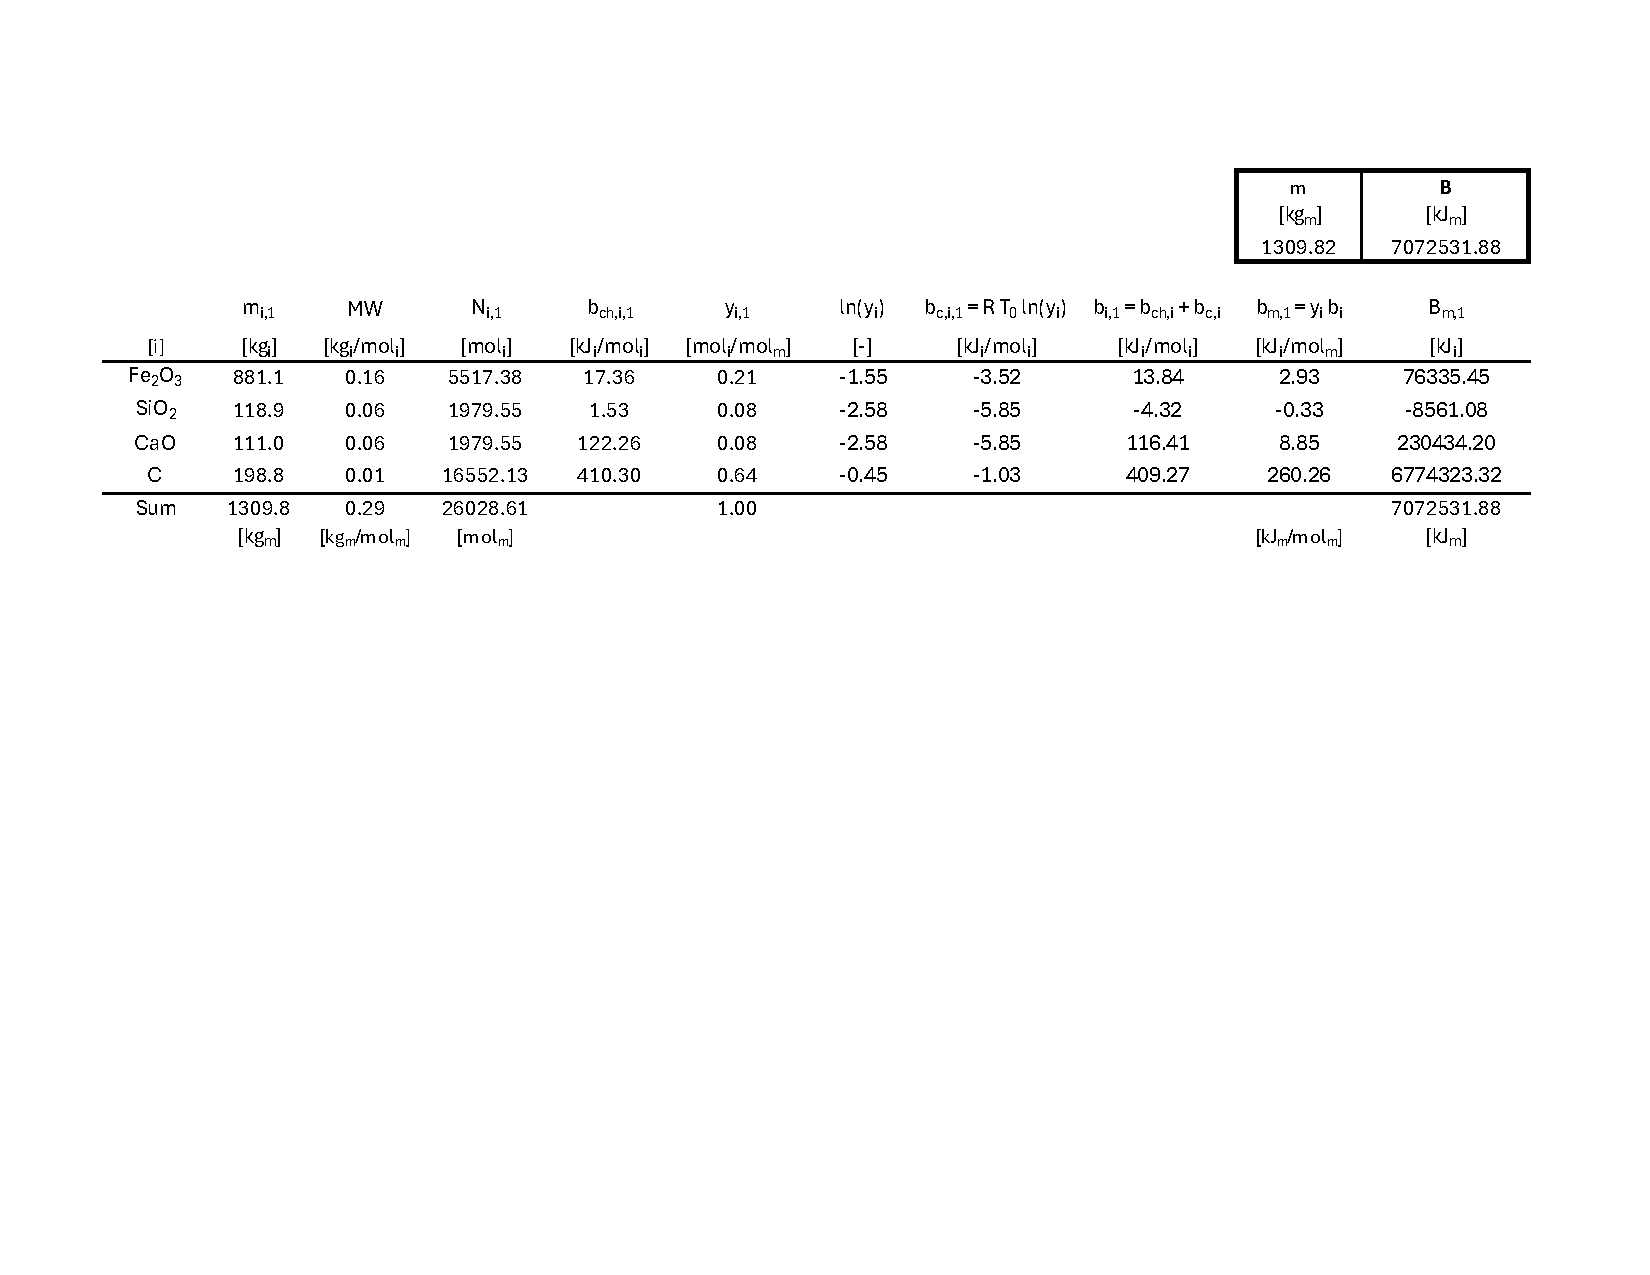
\includegraphics[width=0.8\textwidth]{images/Solid BF Inputs.pdf}
%\end{adjustwidth}
  \caption{Material exergy accounting for the solid blast furnace inputs: iron ore, limestone, and coking coal.}
  \label{fig:Solid Blast Furnace Inputs}
\end{table}

The total material exergy of ore inputs
in Figure~\ref{fig1} is 7072531.88 kJ.
The material exergy in Figure~\ref{fig1}
of hematite ore is 76335.34 kJ.

\begin{table}
%\begin{adjustwidth}{-\extralength}{0cm}
  \centering
  \caption{Material exergy accounting for the gaseous blast furnace inputs: air.}
  \label{fig:Gaseous Blast Furnace Inputs}
  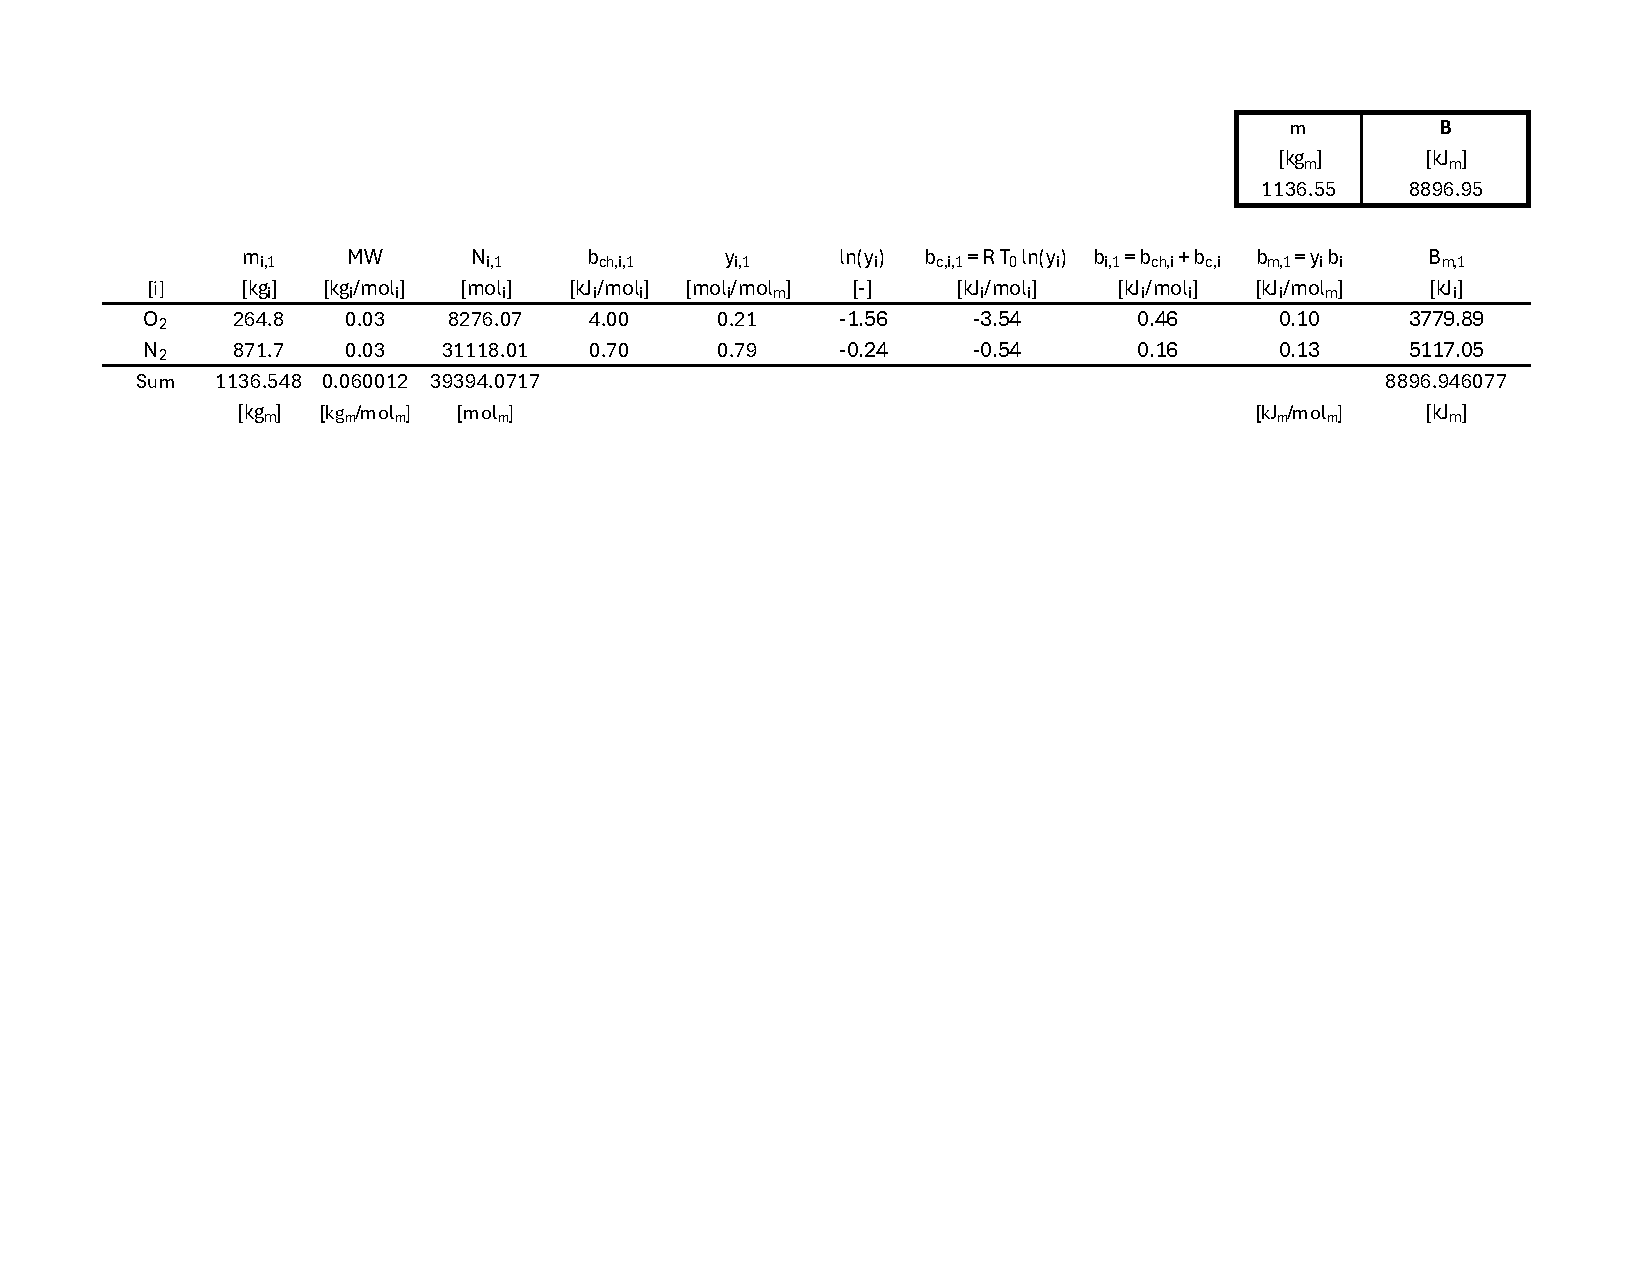
\includegraphics[width=0.8\textwidth]{images/Air BF Inputs.pdf}
%\end{adjustwidth}

\end{table}

The total material exergy of air
in Figure~\ref{fig2} is 8896.95 kJ.


%++++++++++++++++++++++++++++++
\subsection{Efficiency Methods}
%++++++++++++++++++++++++++++++

Three efficiency calculation methods,
seen in Figure~\ref{fig:efficiencymethods},
were applied to the material conversion chain
from mineral extraction
to the blast furnace.
The material and energy exergy
at each statepoint
makes up in exergy in and out
of a process,
like the blast furnace.

\begin{itemize}
  \item The Bejan method focuses on the main product
  at a statepoint
  to quantify how the material's exergy upgraded
  due to concentration of the compound
  by energy exergy inputted.
  \item The Product method focuses on the main product's exergy
  compared to the total exergy used
  at the previous statepoint,
  \item The Student method focuses on the total output
  compared to the total input.
\end{itemize}

\begin{figure}
\centering
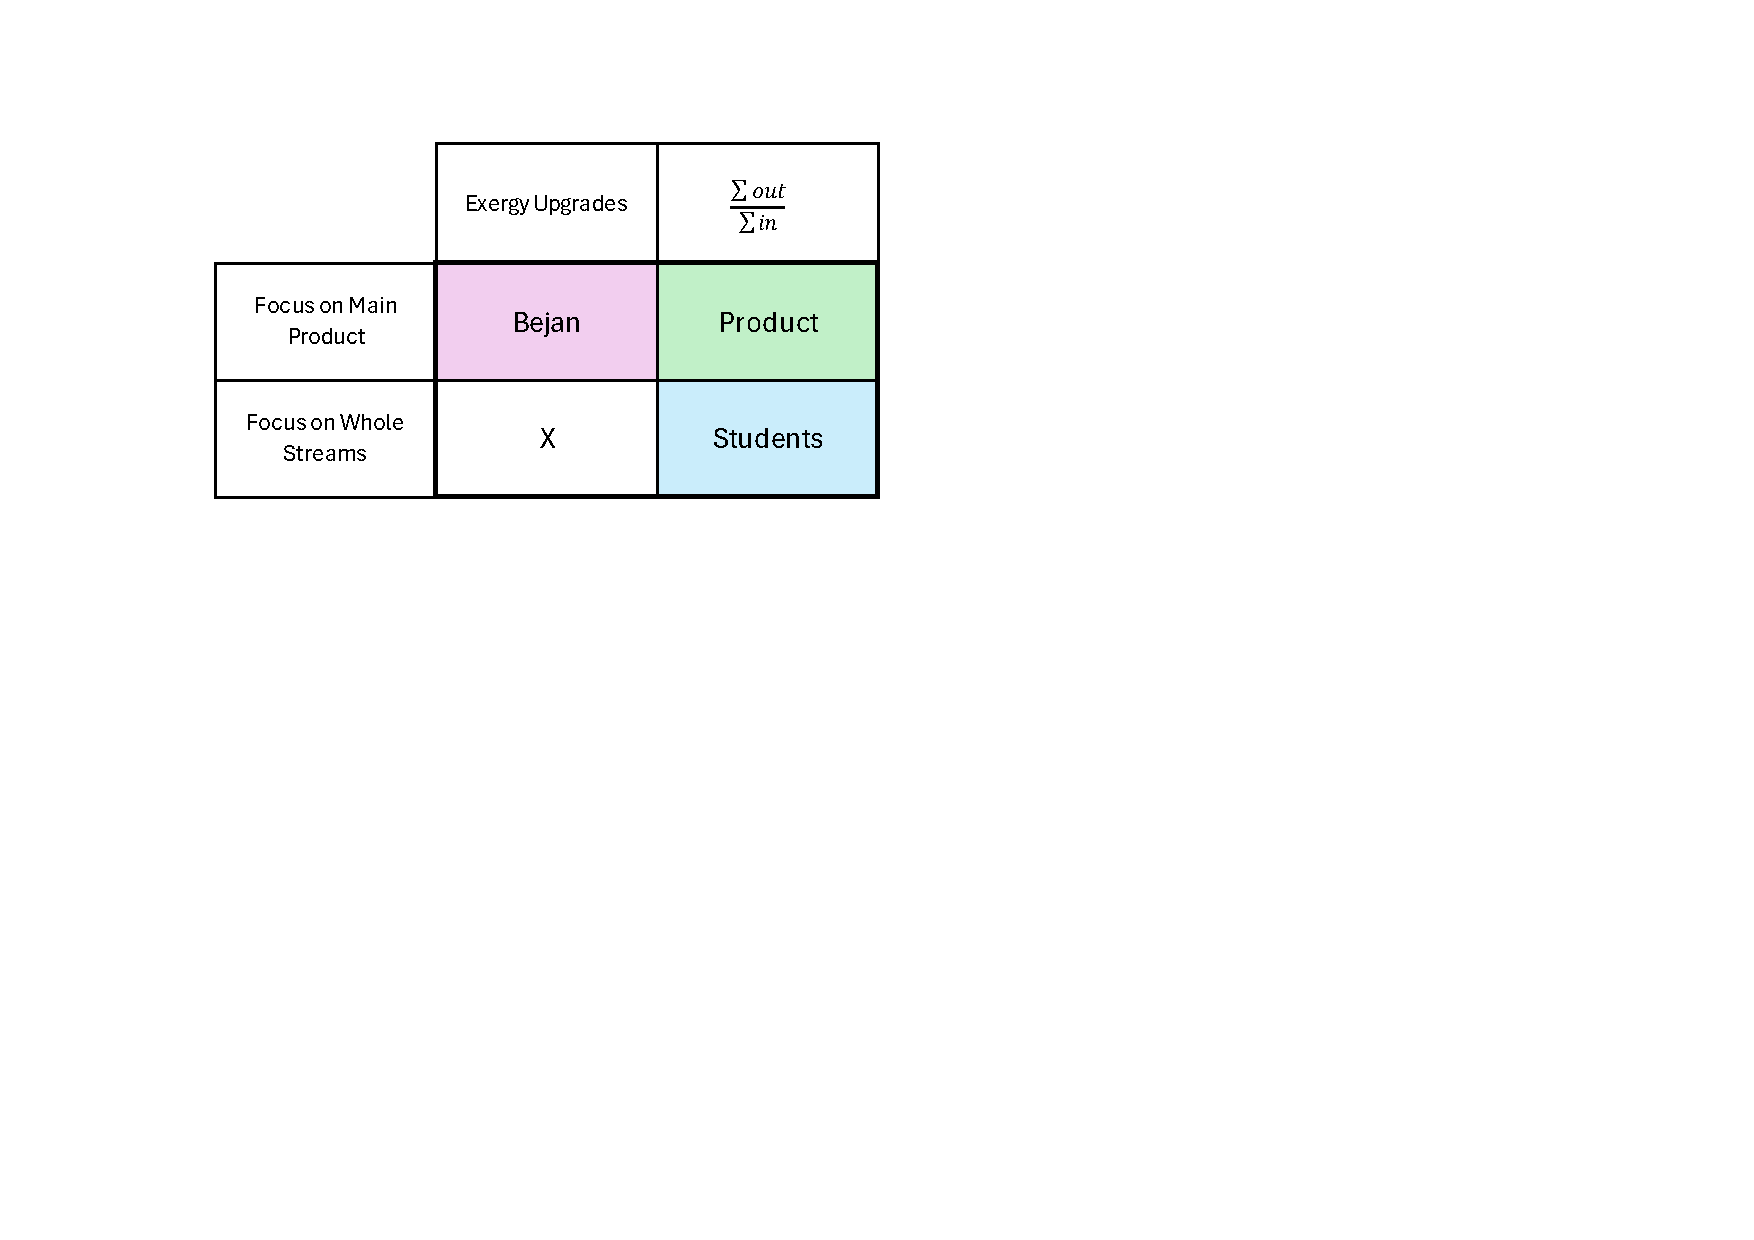
\includegraphics[width=0.8\linewidth]{images/efficiency_methods.pdf}
\caption{Three efficiency methods used for energy and material exergy conversion chains.}
\label{fig:efficiencymethods}
\end{figure}


The Bejan method uses the material exergy ($b_{m,i}$)
of hematite ore, 2.93 kJ as seen in Figure~\ref{fig1},
and compare it to the material exergy
at the next statepoint.
The energy exergy input,
to the blast furnace,
is the work it takes
to concentrate the hematite ore
to pig iron.

The Product method uses the total material exergy ($B$)
of the desired output,
such as pig iron,
and the total material exergy
of all material and energy streams
as the input.
In the blast furnace example,
the total material exergy input
is 7081428.83 kJ.

The Student method uses the total material exergy ($B$)
of all material and energy streams
as the input
and the total material exergy
of all material streams
as the output.

%%%%%%%%%%%%%%%%%%%%%%%%%%%%%%%%%%%%%%%%%%
\section{Discussion}

Authors should discuss the results and how they can be interpreted from the perspective of previous studies and of the working hypotheses. The findings and their implications should be discussed in the broadest context possible. Future research directions may also be highlighted.

%%%%%%%%%%%%%%%%%%%%%%%%%%%%%%%%%%%%%%%%%%
\section{Conclusions}

This section is not mandatory, but can be added to the manuscript if the discussion is unusually long or complex.

%%%%%%%%%%%%%%%%%%%%%%%%%%%%%%%%%%%%%%%%%%
\section{Patents}

This section is not mandatory, but may be added if there are patents resulting from the work reported in this manuscript.

%%%%%%%%%%%%%%%%%%%%%%%%%%%%%%%%%%%%%%%%%%
\vspace{6pt}

%%%%%%%%%%%%%%%%%%%%%%%%%%%%%%%%%%%%%%%%%%
%% optional
%\supplementary{The following supporting information can be downloaded at:  \linksupplementary{s1}, Figure S1: title; Table S1: title; Video S1: title.}

% Only for journal Methods and Protocols:
% If you wish to submit a video article, please do so with any other supplementary material.
% \supplementary{The following supporting information can be downloaded at: \linksupplementary{s1}, Figure S1: title; Table S1: title; Video S1: title. A supporting video article is available at doi: link.}

% Only used for preprtints:
% \supplementary{The following supporting information can be downloaded at the website of this paper posted on \href{https://www.preprints.org/}{Preprints.org}.}

% Only for journal Hardware:
% If you wish to submit a video article, please do so with any other supplementary material.
% \supplementary{The following supporting information can be downloaded at: \linksupplementary{s1}, Figure S1: title; Table S1: title; Video S1: title.\vspace{6pt}\\
%\begin{tabularx}{\textwidth}{lll}
%\toprule
%\textbf{Name} & \textbf{Type} & \textbf{Description} \\
%\midrule
%S1 & Python script (.py) & Script of python source code used in XX \\
%S2 & Text (.txt) & Script of modelling code used to make Figure X \\
%S3 & Text (.txt) & Raw data from experiment X \\
%S4 & Video (.mp4) & Video demonstrating the hardware in use \\
%... & ... & ... \\
%\bottomrule
%\end{tabularx}
%}

%%%%%%%%%%%%%%%%%%%%%%%%%%%%%%%%%%%%%%%%%%
\authorcontributions{For research articles with several authors, a short paragraph specifying their individual contributions must be provided. The following statements should be used ``Conceptualization, X.X. and Y.Y.; methodology, X.X.; software, X.X.; validation, X.X., Y.Y. and Z.Z.; formal analysis, X.X.; investigation, X.X.; resources, X.X.; data curation, X.X.; writing---original draft preparation, X.X.; writing---review and editing, X.X.; visualization, X.X.; supervision, X.X.; project administration, X.X.; funding acquisition, Y.Y. All authors have read and agreed to the published version of the manuscript.'', please turn to the  \href{http://img.mdpi.org/data/contributor-role-instruction.pdf}{CRediT taxonomy} for the term explanation. Authorship must be limited to those who have contributed substantially to the work~reported.}

\funding{Please add: ``This research received no external funding'' or ``This research was funded by NAME OF FUNDER grant number XXX.'' and  and ``The APC was funded by XXX''. Check carefully that the details given are accurate and use the standard spelling of funding agency names at \url{https://search.crossref.org/funding}, any errors may affect your future funding.}

\institutionalreview{In this section, you should add the Institutional Review Board Statement and approval number, if relevant to your study. You might choose to exclude this statement if the study did not require ethical approval. Please note that the Editorial Office might ask you for further information. Please add “The study was conducted in accordance with the Declaration of Helsinki, and approved by the Institutional Review Board (or Ethics Committee) of NAME OF INSTITUTE (protocol code XXX and date of approval).” for studies involving humans. OR “The animal study protocol was approved by the Institutional Review Board (or Ethics Committee) of NAME OF INSTITUTE (protocol code XXX and date of approval).” for studies involving animals. OR “Ethical review and approval were waived for this study due to REASON (please provide a detailed justification).” OR “Not applicable” for studies not involving humans or animals.}

\informedconsent{Any research article describing a study involving humans should contain this statement. Please add ``Informed consent was obtained from all subjects involved in the study.'' OR ``Patient consent was waived due to REASON (please provide a detailed justification).'' OR ``Not applicable'' for studies not involving humans. You might also choose to exclude this statement if the study did not involve humans.

Written informed consent for publication must be obtained from participating patients who can be identified (including by the patients themselves). Please state ``Written informed consent has been obtained from the patient(s) to publish this paper'' if applicable.}

\dataavailability{We encourage all authors of articles published in MDPI journals to share their research data. In this section, please provide details regarding where data supporting reported results can be found, including links to publicly archived datasets analyzed or generated during the study. Where no new data were created, or where data is unavailable due to privacy or ethical restrictions, a statement is still required. Suggested Data Availability Statements are available in section ``MDPI Research Data Policies'' at \url{https://www.mdpi.com/ethics}.}

% Only for journal Drones
%\durcstatement{Current research is limited to the [please insert a specific academic field, e.g., XXX], which is beneficial [share benefits and/or primary use] and does not pose a threat to public health or national security. Authors acknowledge the dual-use potential of the research involving xxx and confirm that all necessary precautions have been taken to prevent potential misuse. As an ethical responsibility, authors strictly adhere to relevant national and international laws about DURC. Authors advocate for responsible deployment, ethical considerations, regulatory compliance, and transparent reporting to mitigate misuse risks and foster beneficial outcomes.}

% Only for journal Nursing Reports
%\publicinvolvement{Please describe how the public (patients, consumers, carers) were involved in the research. Consider reporting against the GRIPP2 (Guidance for Reporting Involvement of Patients and the Public) checklist. If the public were not involved in any aspect of the research add: ``No public involvement in any aspect of this research''.}
%
%% Only for journal Nursing Reports
%\guidelinesstandards{Please add a statement indicating which reporting guideline was used when drafting the report. For example, ``This manuscript was drafted against the XXX (the full name of reporting guidelines and citation) for XXX (type of research) research''. A complete list of reporting guidelines can be accessed via the equator network: \url{https://www.equator-network.org/}.}
%
%% Only for journal Nursing Reports
%\useofartificialintelligence{Please describe in detail any and all uses of artificial intelligence (AI) or AI-assisted tools used in the preparation of the manuscript. This may include, but is not limited to, language translation, language editing and grammar, or generating text. Alternatively, please state that “AI or AI-assisted tools were not used in drafting any aspect of this manuscript”.}

\acknowledgments{In this section you can acknowledge any support given which is not covered by the author contribution or funding sections. This may include administrative and technical support, or donations in kind (e.g., materials used for experiments). Where GenAI has been used for purposes such as generating text, data, or graphics, or for study design, data collection, analysis, or interpretation of data, please add “During the preparation of this manuscript/study, the author(s) used [tool name, version information] for the purposes of [description of use]. The authors have reviewed and edited the output and take full responsibility for the content of this publication.”}

\conflictsofinterest{Declare conflicts of interest or state ``The authors declare no conflicts of interest.'' Authors must identify and declare any personal circumstances or interest that may be perceived as inappropriately influencing the representation or interpretation of reported research results. Any role of the funders in the design of the study; in the collection, analyses or interpretation of data; in the writing of the manuscript; or in the decision to publish the results must be declared in this section. If there is no role, please state ``The funders had no role in the design of the study; in the collection, analyses, or interpretation of data; in the writing of the manuscript; or in the decision to publish the results''.}

%%%%%%%%%%%%%%%%%%%%%%%%%%%%%%%%%%%%%%%%%%
%% Optional

%% Only for journal Encyclopedia
%\entrylink{The Link to this entry published on the encyclopedia platform.}

\abbreviations{Abbreviations}{
The following abbreviations are used in this manuscript:
\\

\noindent
\begin{tabular}{@{}ll}
MDPI & Multidisciplinary Digital Publishing Institute\\
DOAJ & Directory of open access journals\\
TLA & Three letter acronym\\
LD & Linear dichroism
\end{tabular}
}

%%%%%%%%%%%%%%%%%%%%%%%%%%%%%%%%%%%%%%%%%%
%% Optional
\appendixtitles{no} % Leave argument "no" if all appendix headings stay EMPTY (then no dot is printed after "Appendix A"). If the appendix sections contain a heading then change the argument to "yes".
\appendixstart
\appendix
\section[\appendixname~\thesection]{}
\subsection[\appendixname~\thesubsection]{}
The appendix is an optional section that can contain details and data supplemental to the main text---for example, explanations of experimental details that would disrupt the flow of the main text but nonetheless remain crucial to understanding and reproducing the research shown; figures of replicates for experiments of which representative data are shown in the main text can be added here if brief, or as Supplementary Data. Mathematical proofs of results not central to the paper can be added as an appendix.

\begin{table}[H]
\caption{This is a table caption.\label{tab5}}
%\newcolumntype{C}{>{\centering\arraybackslash}X}
\begin{tabularx}{\textwidth}{CCC}
\toprule
\textbf{Title 1}	& \textbf{Title 2}	& \textbf{Title 3}\\
\midrule
Entry 1		& Data			& Data\\
Entry 2		& Data			& Data\\
\bottomrule
\end{tabularx}
\end{table}

\section[\appendixname~\thesection]{}
All appendix sections must be cited in the main text. In the appendices, Figures, Tables, etc. should be labeled, starting with ``A''---e.g., Figure A1, Figure A2, etc.

%%%%%%%%%%%%%%%%%%%%%%%%%%%%%%%%%%%%%%%%%%
%\isPreprints{} % If the paper is ``preprints'', please uncomment this parenthesis.
%\printendnotes[custom] % Un-comment to print a list of endnotes

\reftitle{References}

% Please provide either the correct journal abbreviation (e.g. according to the “List of Title Word Abbreviations” http://www.issn.org/services/online-services/access-to-the-ltwa/) or the full name of the journal.
% Citations and References in Supplementary files are permitted provided that they also appear in the reference list here.

%=====================================
% References, variant A: external bibliography
%=====================================
% \bibliography{your_external_BibTeX_file}

%=====================================
% References, variant B: internal bibliography
%=====================================

% ACS format
\isAPAandChicago{}{%
\begin{thebibliography}{999}
% Reference 1
\bibitem[Author1(year)]{ref-journal}
Author~1, T. The title of the cited article. {\em Journal Abbreviation} {\bf 2008}, {\em 10}, 142--149.
% Reference 2
\bibitem[Author2(year)]{ref-book1}
Author~2, L. The title of the cited contribution. In {\em The Book Title}; Editor 1, F., Editor 2, A., Eds.; Publishing House: City, Country, 2007; pp. 32--58.
% Reference 3
\bibitem[Author1 and Author2 (year)]{ref-book2}
Author 1, A.; Author 2, B. \textit{Book Title}, 3rd ed.; Publisher: Publisher Location, Country, 2008; pp. 154--196.
% Reference 4
\bibitem[Author4(year)]{ref-unpublish}
Author 1, A.B.; Author 2, C. Title of Unpublished Work. \textit{Abbreviated Journal Name} year, \textit{phrase indicating stage of publication (submitted; accepted; in press)}.
% Reference 5
\bibitem[Author8(year)]{ref-url}
Title of Site. Available online: URL (accessed on Day Month Year).
% Reference 6
\bibitem[Author6(year)]{ref-proceeding}
Author 1, A.B.; Author 2, C.D.; Author 3, E.F. Title of presentation. In Proceedings of the Name of the Conference, Location of Conference, Country, Date of Conference (Day Month Year); Abstract Number (optional), Pagination (optional).
% Reference 7
\bibitem[Author7(year)]{ref-thesis}
Author 1, A.B. Title of Thesis. Level of Thesis, Degree-Granting University, Location of University, Date of Completion.
\end{thebibliography}
}

% Chicago format (Used for journal: arts, genealogy, histories, humanities, jintelligence, laws, literature, religions, risks, socsci)
\isChicagoStyle{%
\begin{thebibliography}{999}
% Reference 1
\bibitem[Aranceta-Bartrina(1999a)]{ref-journal}
Aranceta-Bartrina, Javier. 1999a. Title of the cited article. \textit{Journal Title} 6: 100--10.
% Reference 2
\bibitem[Aranceta-Bartrina(1999b)]{ref-book1}
Aranceta-Bartrina, Javier. 1999b. Title of the chapter. In \textit{Book Title}, 2nd ed. Edited by Editor 1 and Editor 2. Publication place: Publisher, vol. 3, pp. 54–96.
% Reference 3
\bibitem[Baranwal and Munteanu {[1921]}(1955)]{ref-book2}
Baranwal, Ajay K., and Costea Munteanu. 1955. \textit{Book Title}. Publication place: Publisher, pp. 154--96. First published 1921 (op-tional).
% Reference 4
\bibitem[Berry and Smith(1999)]{ref-thesis}
Berry, Evan, and Amy M. Smith. 1999. Title of Thesis. Level of Thesis, Degree-Granting University, City, Country. Identifi-cation information (if available).
% Reference 5
\bibitem[Cojocaru et al.(1999)]{ref-unpublish}
Cojocaru, Ludmila, Dragos Constatin Sanda, and Eun Kyeong Yun. 1999. Title of Unpublished Work. \textit{Journal Title}, phrase indicating stage of publication.
% Reference 6
\bibitem[Driver et al.(2000)]{ref-proceeding}
Driver, John P., Steffen Rohrs, and Sean Meighoo. 2000. Title of Presentation. In \textit{Title of the Collected Work} (if available). Paper presented at Name of the Conference, Location of Conference, Date of Conference.
% Reference 7
\bibitem[Harwood(2008)]{ref-url}
Harwood, John. 2008. Title of the cited article. Available online: URL (accessed on Day Month Year).
\end{thebibliography}
}{}

% APA format (Used for journal: admsci, behavsci, businesses, econometrics, economies, education, ejihpe, games, humans, ijfs, journalmedia, jrfm, languages, psycholint, publications, tourismhosp, youth)
\isAPAStyle{%
\begin{thebibliography}{999}
% Reference 1
\bibitem[\protect\citeauthoryear{Azikiwe \BBA\ Bello}{{2020a}}]{ref-journal}
Azikiwe, H., \& Bello, A. (2020a). Title of the cited article. \textit{Journal Title}, \textit{Volume}(Issue),
Firstpage--Lastpage/Article Number.
% Reference 2
\bibitem[\protect\citeauthoryear{Azikiwe \BBA\ Bello}{{2020b}}]{ref-book1}
Azikiwe, H., \& Bello, A. (2020b). \textit{Book title}. Publisher Name.
% Reference 3
\bibitem[Davison(1623/2019)]{ref-book2}
Davison, T. E. (2019). Title of the book chapter. In A. A. Editor (Ed.), \textit{Title of the book: Subtitle}
(pp. Firstpage--Lastpage). Publisher Name. (Original work published 1623) (Optional).
% Reference 4
\bibitem[Fistek et al.(2017)]{ref-proceeding}
Fistek, A., Jester, E., \& Sonnenberg, K. (2017, Month Day). Title of contribution [Type of contribution]. Conference Name, Conference City, Conference Country.
% Reference 5
\bibitem[Hutcheson(2012)]{ref-thesis}
Hutcheson, V. H. (2012). \textit{Title of the thesis} [XX Thesis, Name of Institution Awarding the Degree].
% Reference 6
\bibitem[Lippincott \& Poindexter(2019)]{ref-unpublish}
Lippincott, T., \& Poindexter, E. K. (2019). \textit{Title of the unpublished manuscript} [Unpublished manuscript/Manuscript in prepara-tion/Manuscript submitted for publication]. Department Name, Institution Name.
% Reference 7
\bibitem[Harwood(2008)]{ref-url}
Harwood, J. (2008). \textit{Title of the cited article}. Available online: URL (accessed on Day Month Year).
\end{thebibliography}
}{}

% If authors have biography, please use the format below
%\section*{Short Biography of Authors}
%\bio
%{\raisebox{-0.35cm}{\includegraphics[width=3.5cm,height=5.3cm,clip,keepaspectratio]{Definitions/author1.pdf}}}
%{\textbf{Firstname Lastname} Biography of first author}
%
%\bio
%{\raisebox{-0.35cm}{\includegraphics[width=3.5cm,height=5.3cm,clip,keepaspectratio]{Definitions/author2.jpg}}}
%{\textbf{Firstname Lastname} Biography of second author}

% For the MDPI journals use author-date citation, please follow the formatting guidelines on http://www.mdpi.com/authors/references
% To cite two works by the same author: \citeauthor{ref-journal-1a} (\citeyear{ref-journal-1a}, \citeyear{ref-journal-1b}). This produces: Whittaker (1967, 1975)
% To cite two works by the same author with specific pages: \citeauthor{ref-journal-3a} (\citeyear{ref-journal-3a}, p. 328; \citeyear{ref-journal-3b}, p.475). This produces: Wong (1999, p. 328; 2000, p. 475)

%%%%%%%%%%%%%%%%%%%%%%%%%%%%%%%%%%%%%%%%%%
%% for journal Sci
%\reviewreports{\\
%Reviewer 1 comments and authors’ response\\
%Reviewer 2 comments and authors’ response\\
%Reviewer 3 comments and authors’ response
%}
%%%%%%%%%%%%%%%%%%%%%%%%%%%%%%%%%%%%%%%%%%
\PublishersNote{}
%\isPreprints{} % If the paper is ``preprints'', please uncomment this parenthesis.
\end{document}

